
\section*{\Large\centering \textbf{CHAPTER 1 \\ INTRODUCTION }}
\addcontentsline{toc}{section}{CHAPTER 1: Introduction}
\setcounter{section}{1}

\subsection{Introduction}
Brain tumors are among the most lethal forms of cancer, contributing to high
mortality and morbidity rates worldwide. Early and accurate detection plays a
vital role in improving patient outcomes, as timely treatment significantly
enhances survival rates. However, traditional methods of diagnosis, such as
manual \gls{mri} analysis, prove to be time-consuming, laborious, and
error-prone. In recent years, significant progression has been witnessed in the
field of Artificial Intelligence, and deep learning, in particular, shows great
promise in overcoming these limitations.

In the field of intelligent automation and high accuracy for discriminating
brain tumor presence from medical images, Convolutional Neural Networks, or
\gls{cnn}s, demonstrate remarkable potential. This research discusses the brain
tumor detection and classification problem. It provides an automated approach
to identify the position, size, and shape of tumors through deep learning
techniques applied to medical images. Numerous studies have been undertaken
using machine learning and deep learning techniques for this purpose, with
\gls{cnn}-based models consistently demonstrating some of the most effective
results in medical image analysis.

\subsection{Problem Statement}
Critical and life-threatening diseases such as brain tumors necessitate prompt
and accurate detection to ensure patient survival and maximize treatment
effectiveness. Most conventional diagnostic procedures for these conditions
rely heavily on manual analysis of \gls{mri} scans by experienced radiologists.
These traditional implementations are inherently time-consuming and
error-prone, often yielding inconsistent results, particularly during the
critical early detection stages. The situation has been further complicated by
the exponential surge in medical imaging data volumes, placing unprecedented
pressure on healthcare systems worldwide. There is a clear and urgent need for
automation to develop accurate and efficient systems that can assist healthcare
professionals in making informed decisions about brain tumor detection and
classification.

\subsection{Objectives}
The primary objective of this research is to design and implement a
sophisticated convolutional neural network (\gls{cnn}) model that incorporates
transfer learning techniques with the \gls{vgg16} architecture to enhance
classification accuracy. This model is specifically tailored for precise brain
tumor detection and classification from \gls{mri} images, aiming to provide
reliable automated assistance in medical diagnosis.

\subsection{Scope and Limitation}
The scope of this research encompasses comprehensive preprocessing of medical
images, systematic training of the \gls{cnn} model on various available
datasets, and thorough evaluation of its performance using well-established
metrics including accuracy, precision, recall, and F1-score. This research
emphasizes the transformative role of artificial intelligence in reducing human
error and accelerating diagnostic processes, thereby significantly improving
patient outcomes and healthcare efficiency.

However, this research acknowledges several important limitations. The accuracy
and reliability of the system are inherently influenced by the quality,
diversity, and representativeness of the dataset used for training the neural
network. Given that the datasets employed in this research are limited to
available \gls{mri} scans, the variability may not fully capture the complete
spectrum of differences in tumor types, stages, or imaging conditions
encountered in diverse clinical scenarios.

Furthermore, this model is developed primarily for academic research purposes
and experimental validation. It should not be considered as a replacement for
professional medical judgment or clinical expertise. Additional considerations
include hardware computational constraints, model generalization capabilities
across different populations, and the complex ethical implications surrounding
the use of \gls{ai} in critical medical decision-making processes. These
considerations extend beyond the immediate scope of this study.

\subsection{Development Methodology}
\textbf{Iterative and Incremental Model}

For the successful execution of this project, the Iterative and Incremental Development Model has been adopted. This model is particularly well-suited for projects involving machine learning and deep learning, where experimentation, continuous refinement, and frequent testing are essential. In this approach, the system is built gradually through repeated cycles (iterations), where each cycle results in a functional version of the system. This allows for early evaluation of the model's performance and provides opportunities to identify and correct issues, such as data imbalance or underfitting, in earlier stages. Each iteration adds new features or improvements while preserving the core functionality developed in previous cycles.

The iterative model is especially beneficial for deep learning projects like brain tumor detection and classification, where model architecture, data preprocessing techniques, and hyperparameters often require multiple rounds of testing and fine-tuning. It enables the team to begin with a basic \gls{cnn} implementation and progressively improve the system by integrating advanced techniques such as transfer learning using \gls{vgg16}. Moreover, this model promotes adaptability, allowing changes in design based on validation feedback and model accuracy. It also facilitates parallel development of modules such as data preparation, model training, evaluation, and documentation, ensuring steady progress and reducing overall project risk.
\begin{figure}[h]
    \centering
    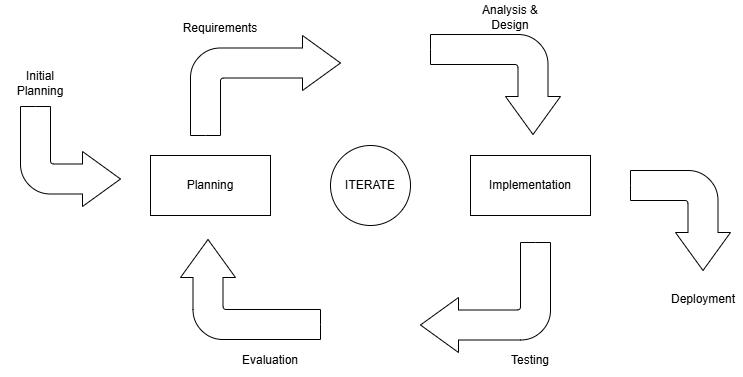
\includegraphics[width=1\linewidth]{Images/model.png}
    \caption{Iterative and Incremental model}
    \label{fig:enter-label}
\end{figure}

